%!TEX TS-program = xelatex
%!TEX encoding = UTF-8 Unicode

\documentclass[12pt]{extarticle}
% extarticle is like article but can handle 8pt, 9pt, 10pt, 11pt, 12pt, 14pt, 17pt, and 20pt text

\def \ititle {Philosophical Psychology}

\def \isubtitle {Lecture 07}

\def \iauthor {Stephen A. Butterfill}
\def \iemail{s.butterfill@warwick.ac.uk}
\date{}

%for strikethrough
\usepackage[normalem]{ulem}

\input{$HOME/latex_imports/preamble_steve_handout}

%\bibpunct{}{}{,}{s}{}{,}  %use superscript TICS style bib
%remove hanging indent for TICS style bib
%TODO doesnt work
\setlength{\bibhang}{0em}
%\setlength{\bibsep}{0.5em}


%itemize bullet should be dash
\renewcommand{\labelitemi}{$-$}

\begin{document}

\begin{multicols*}{3}

\setlength\footnotesep{1em}


\bibliographystyle{newapa} %apalike

%\maketitle
%\tableofcontents




%---------------
%--- start paste




\def \ititle {Lecture 07: A Dual-Process Theory of Mindreading}

\begin{center}

{\Large

\textbf{\ititle}

}



\iemail %

\end{center}

\section{Three Questions}

Q1: What do infants, chimps and scrub-jays reason about, or represent, that enables them, within limits, to track others’ perceptions, knowledge, beliefs and other propositional attitudes?

Q2: Why do infants manifest abilities to track beliefs in some cases but not all?

Q3: Why is belief-tracking in adults sometimes but not always automatic?
(And how could belief-tracking ever be automatic if it significantly depends on working memory and consumes attention?)


\section{Dual-process Theory}

\begin{center}
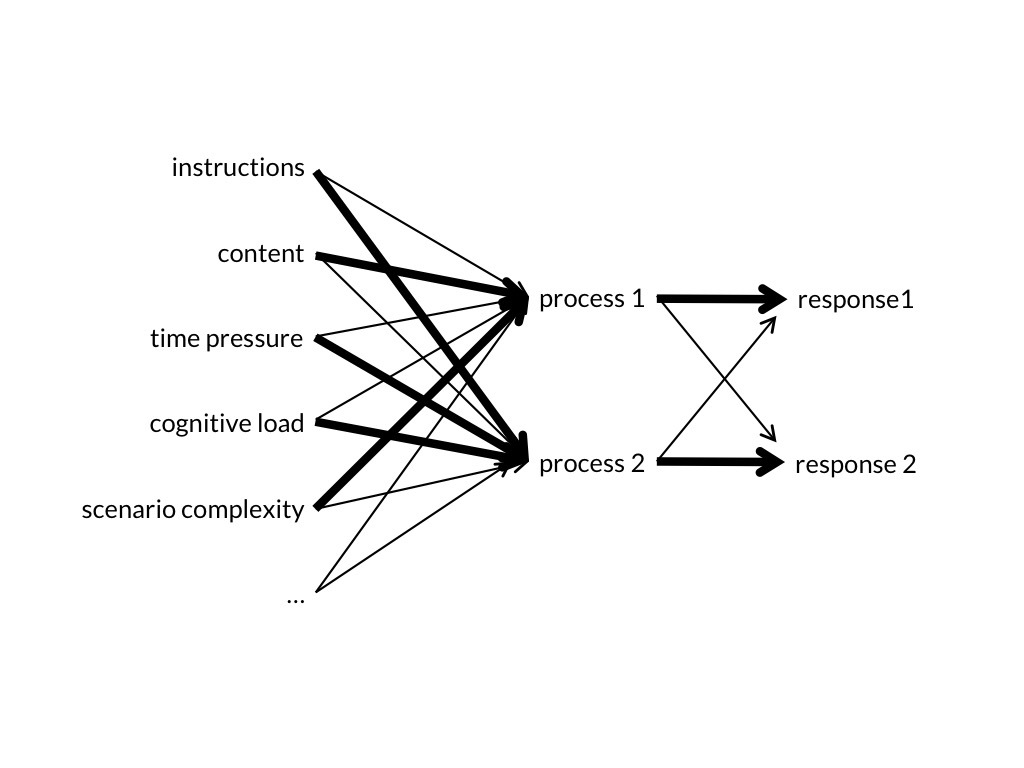
\includegraphics[scale=0.3]{img/dual_process_operationalized_11.neg.jpg}
\end{center}

\emph{Dual Process Theory (core part)}:
Two (or more) processes for tracking Xs are distinct:
the conditions which influence whether they occur,
and which outputs they generate,
do not completely overlap.



\section{Minimal Theory of Mind}

An agent’s \emph{field} is a set of objects related to the agent by proximity, orientation and other factors.

First approximation: an agent \emph{encounters} an object just if it is in her field.

A \emph{goal} is an outcome to which one or more actions are, or might be, directed.

%(Not to be confused with a \emph{goal-state}, which is an intention or other state of an agent linking an action to a particular goal to which it is directed.)

\textbf{Principle 1}: one can’t goal-directedly act on an object unless one has encountered it.

Applications: subordinate chimps retrieve food when a dominant is not informed of its
          location \citep{Hare:2001ph}; when observed scrub-jays prefer to cache in shady, distant and
          occluded locations \citep{Dally:2004xf,Clayton:2007fh}.

First approximation: an agent \emph{registers} an object at a location just if she most recently encountered the object at that location.

A registration is \emph{correct} just if the object is at the location it is registered at.

\textbf{Principle 2}: correct registration is a condition of successful action.

Applications: 12-month-olds point to inform depending on their informants’ goals and ignorance \citep{Liszkowski:2008al};
          chimps retrieve food when a dominant is misinformed about its location \citep{Hare:2001ph};
          scrub-jays observed caching food by a competitor later re-cache in private \citep{Clayton:2007fh,Emery:2007ze}.

\textbf{Principle 3}: when an agent performs a goal-directed action and the goal specifies an object, the agent will act as if the object were actually in the location she registers it at.

Applications: some false belief tasks \citep{Onishi:2005hm,Southgate:2007js,Buttelmann:2009gy}.




\section{Signature Limits}
A \emph{signature limit of a model} is a set of predictions derivable from the model which are
incorrect, and which are not predictions of other models under consideration.
(See \citealp{wang:2015_limits,low:2010_preschoolers,low:2014_quack,edwards:2017_reaction}; contrast \citealp{scott:2015_infants}.)


Automatic belief-tracking in adults and
belief-tracking in infants are both subject to signature limits
associated with minimal theory of mind
(\citealp{wang:2015_limits,Low:2012_identity,low:2014_quack,mozuraitis:2015_privileged};
contrast \citealp{scott:2015_infants}).

\begin{center}

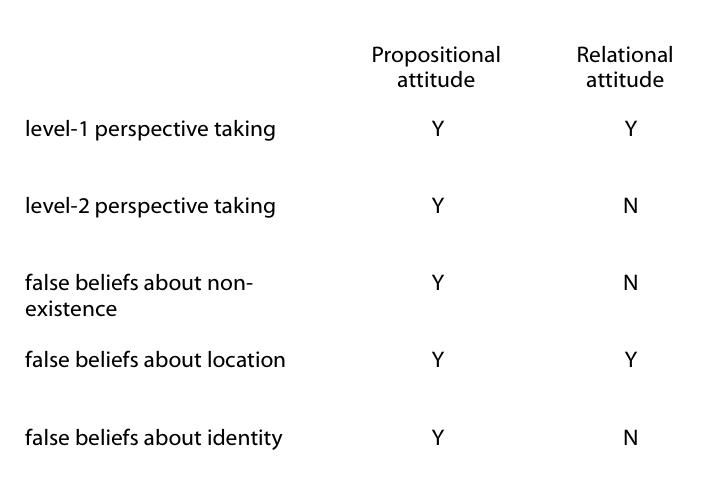
\includegraphics[width=0.25\textwidth]{fig/signature_limits_table.png}

\end{center}

\begin{center}

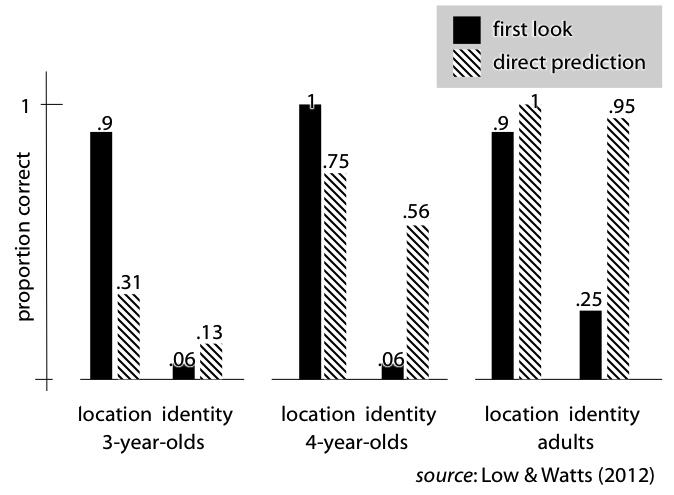
\includegraphics[width=0.3\textwidth]{fig/low_2012_fig.png}

\end{center}

For adults (and children who can do this),
representing perceptions and beliefs as such---and even merely holding in mind
what another believes, where no inference is required---involves a measurable
processing cost \citep{apperly:2008_back,apperly:2010_limits}, consumes attention
and working memory in fully competent adults \citealp{Apperly:2009cc,
lin:2010_reflexively, McKinnon:2007rr},  may require inhibition \citep{bull:2008_role}
and makes demands on executive function \citep{apperly:2004_frontal,samson:2005_seeing}.


\section{Objections}
‘the theoretical arguments offered [...] are [...] unconvincing, and [...]
the data can be explained in other terms’
(\citealp{carruthers:2015_two}; see also \citealp{carruthers:2015_mindreading}).

‘A cooperative multi-system architecture is better able to explain infant belief representation than a
parallel architecture, and causal representation, schemas and models provide a more promising basis
for flexible belief representation than does a rule-based approach of the kind described by Butterfill
and Apperly’ (\citealp{christensen:_twoa}; see also \citealp{michael:2016_flexible,michael:2013_mindreading}).

\section{What about Development?}
\begin{enumerate}
\item Automatic and nonautomatic mindreading processes both occur from the first year of life onwards.
\item The model of minds and actions underpinning automatic mindreading process does not
significantly change over development.
\item In the first three or four years of life, nonautomatic mindreading processes involve
relatively crude models of minds and actions, models which do not enable belief tracking.
\item What changes over development is typically just that the model underpinning nonautomatic
mindreading becomes gradually more sophisticated and eventually comes to enable belief tracking.
\end{enumerate}




\section{Maymon, Sivanantham, Low \& Butterfill (pilot)}

\begin{center}
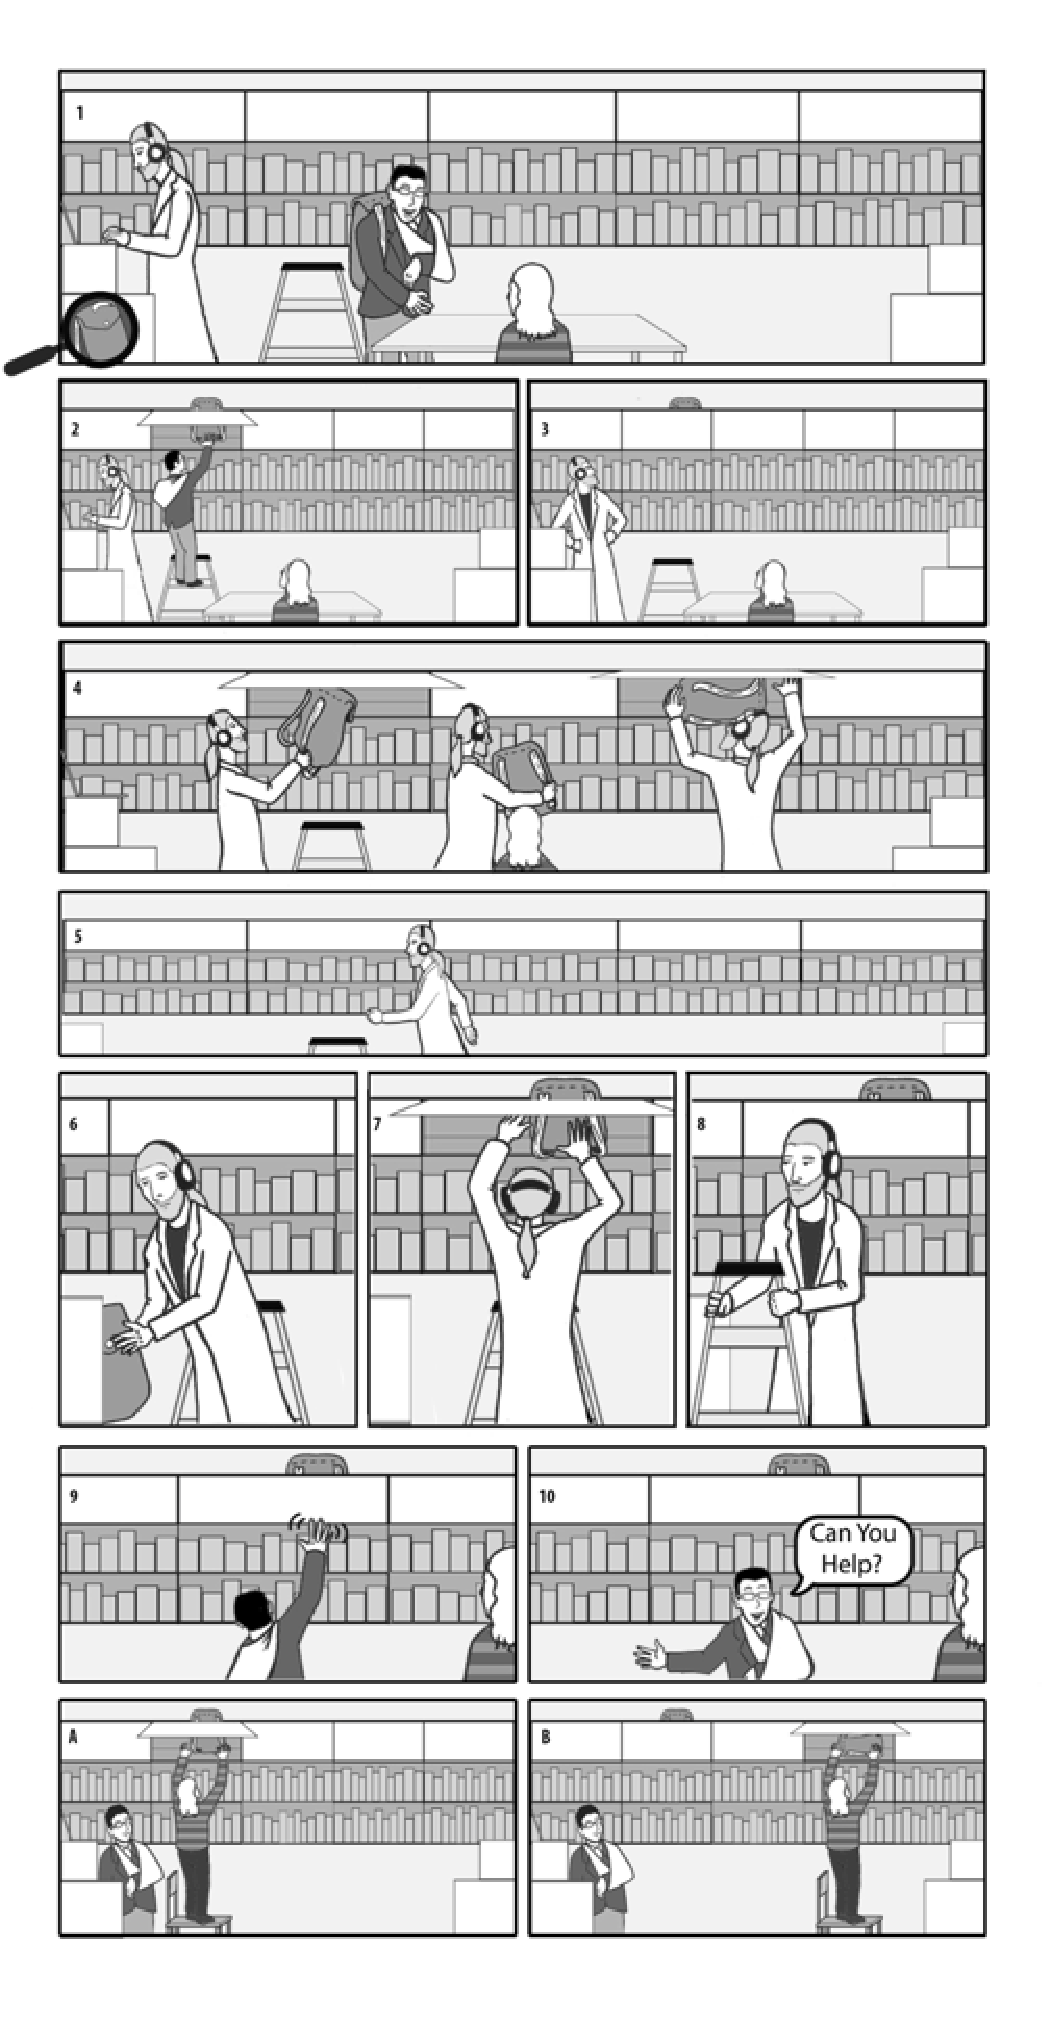
\includegraphics[scale=0.37]{img/maymon_fig1.png}
\end{center}
Sequence of events (1 – 10) in the FB-identity condition.

\
\begin{center}
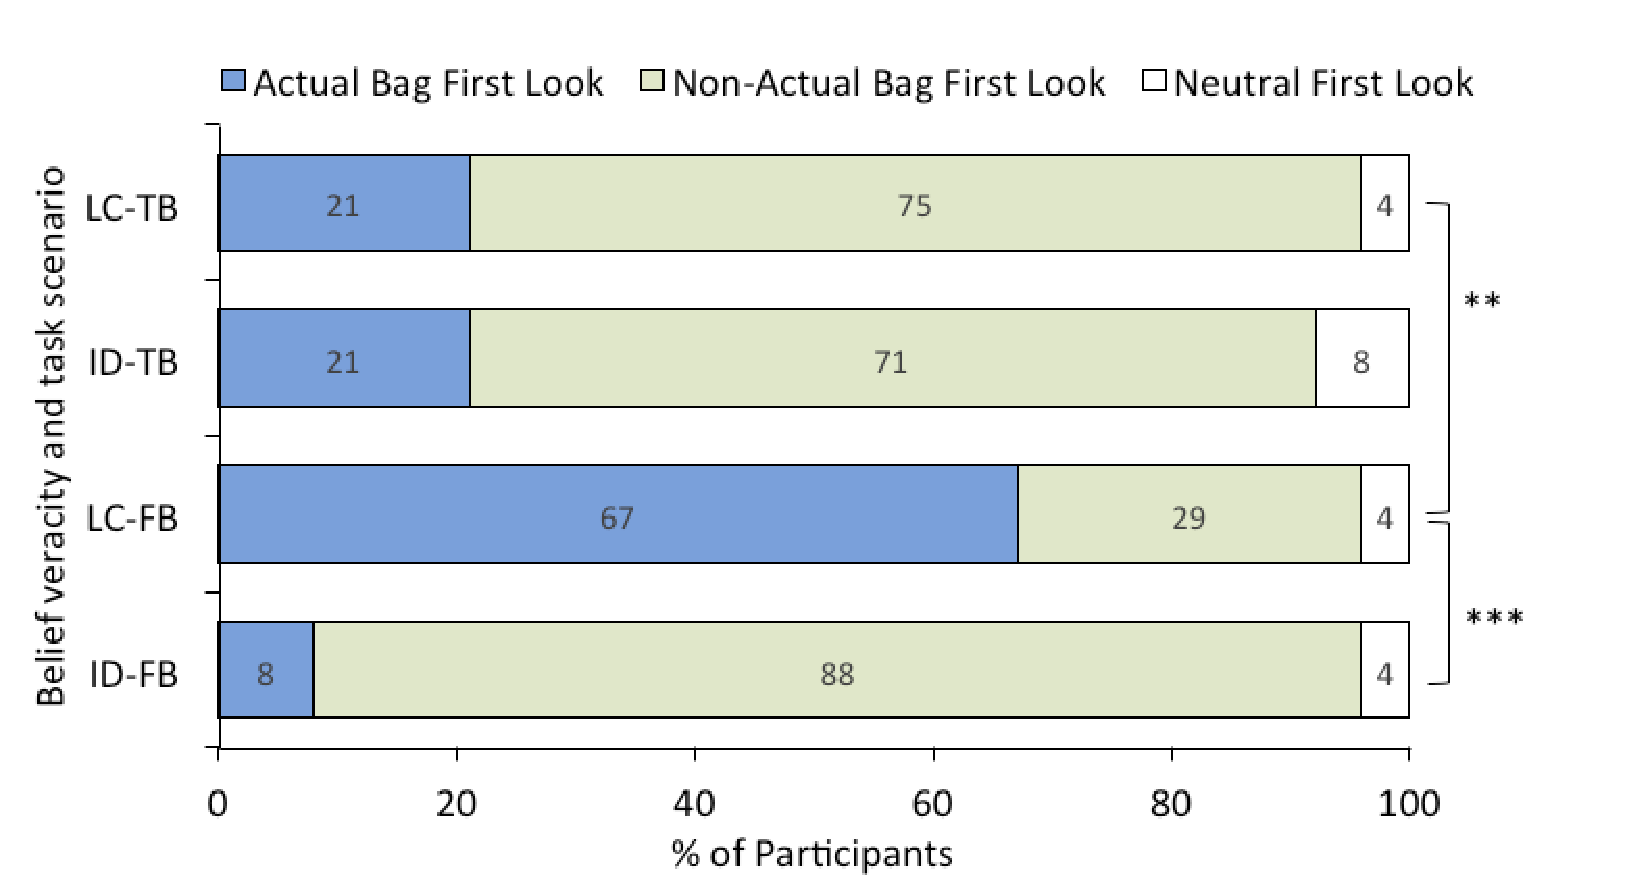
\includegraphics[scale=0.3]{img/maymon_fig3.png}
\end{center}
\% of participants displaying type of first look by condition (**P = 0.005; ***P < 0.001).

\vfill


\ 

\columnbreak

\begin{center}
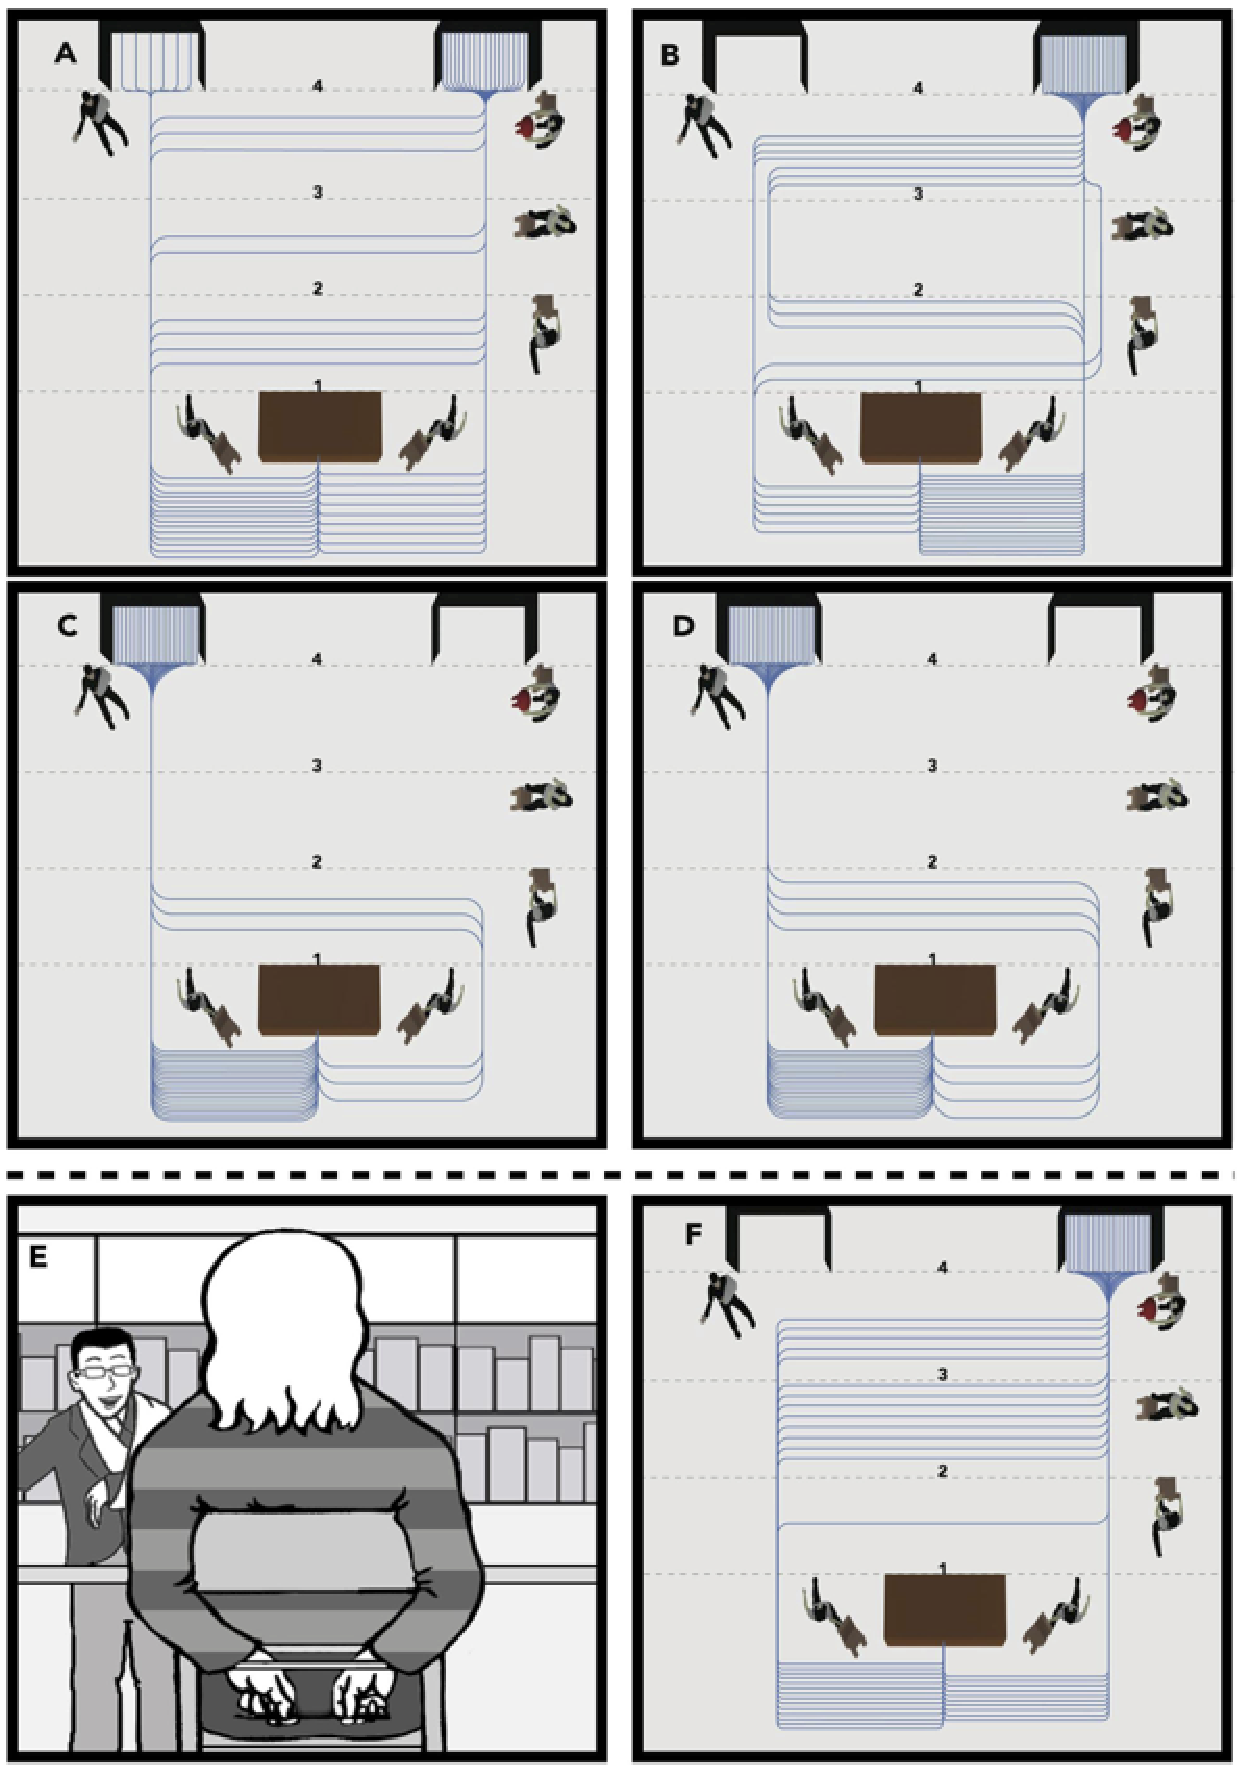
\includegraphics[scale=0.33]{img/maymon_fig4.png}
\end{center}

Schematic representation of individuals’ (N = 96) course of action in Experiment 1 between conditions: (A) FB-identity, (B) FB-location, (C) TB-identity, and (D) TB-location. The course was divided into 4 stages: (1) swerving, (2) advancing, (3) reaching, and (4) ultimately handing over the actual or non-actual bag (dotted lines represent thresholds for each stage). In Experiment 2, we examined how stalling of motor representations, by temporarily tying individual observers’ hands (E), affected the course of their (N = 24) helping action in the FB-location condition (F).


%--- end paste
%---------------

\footnotesize
\bibliography{$HOME/endnote/phd_biblio}

\end{multicols*}

\end{document}
